% Oversells — ish varagʻi shabloni (XeLaTeX).
% Worksheet template (compile with XeLaTeX or LuaLaTeX).
\documentclass[12pt,a4paper]{article}

\usepackage[margin=2cm, headheight=15pt]{geometry}
\usepackage{fontspec}
\setmainfont{Noto Serif}
\setsansfont{Noto Sans}
\usepackage{babel}
\babelprovide[import=uz-Latn, main]{uzbek}
\setlength{\emergencystretch}{3em}

\usepackage{amsmath, amssymb}
\usepackage{enumitem}
\usepackage{tikz}
\usepackage{fancyhdr}

\pagestyle{fancy}
\fancyhf{}
\lhead{\sffamily Matematika, 7-sinf}
\rhead{\sffamily Ish varagʻi №\,1}
\cfoot{\thepage}

% Javob uchun chiziqlar / lines for answers
\newcommand{\javob}[1][2]{%
  \par\vspace{0.3em}%
  \foreach \i in {1,...,#1}{\noindent\rule{\linewidth}{0.4pt}\par\vspace{0.9em}}%
}

\begin{document}

\begin{center}
  {\Large\sffamily\bfseries Chiziqli tenglamalar}\\[0.5em]
  {\sffamily Mustaqil ish}
\end{center}

\noindent
\begin{tabular}{@{}p{0.55\linewidth}p{0.4\linewidth}@{}}
  Familiya, ism: \hrulefill & Sinf: \hrulefill \\[0.6em]
  Sana: \hrulefill & Baho: \hrulefill
\end{tabular}

\section*{1-topshiriq. Tenglamani yeching}

\begin{enumerate}[label=\alph*), itemsep=0.5em]
  \item $3x + 5 = 20$ \javob[1]
  \item $2(x - 4) = x + 1$ \javob[1]
  \item $\dfrac{x}{3} - 2 = 4$ \javob[1]
\end{enumerate}

\section*{2-topshiriq. Masala}

Doʻkonda daftar $x$ soʻm, ruchka esa undan $1500$ soʻm qimmat turadi.
Oʻquvchi $3$ ta daftar va $2$ ta ruchka uchun $18\,000$ soʻm toʻladi.
Daftar necha soʻm turadi?
\javob[3]

\section*{3-topshiriq. Grafikni chizing}

$y = 2x - 1$ funksiyaning grafigini koordinata tekisligida chizing.

\begin{center}
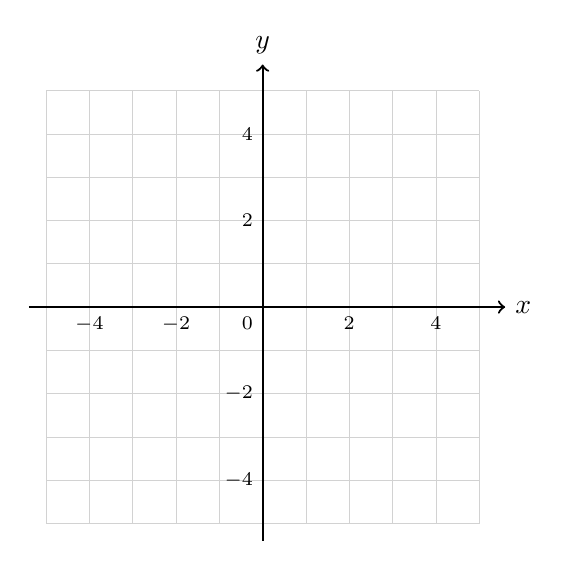
\begin{tikzpicture}[scale=0.55]
  \draw[step=1, gray!35, very thin] (-5,-5) grid (5,5);
  \draw[->, thick] (-5.4,0) -- (5.6,0) node[right] {$x$};
  \draw[->, thick] (0,-5.4) -- (0,5.6) node[above] {$y$};
  \foreach \k in {-4,-2,2,4} {
    \node[below, font=\scriptsize] at (\k,0) {$\k$};
    \node[left, font=\scriptsize] at (0,\k) {$\k$};
  }
  \node[below left, font=\scriptsize] at (0,0) {$0$};
\end{tikzpicture}
\end{center}

\end{document}
